\utsection{Einleitung}{Stefan Giggenbach}

Im Rahmen des Moduls Mobile Netze im Masterstudiengang Informatik wird mit der Durchführung einer Projektarbeit, dass in der Vorlesung vermittelte Wissen praxisnah vertieft und  ergänzt. In der vorliegenden Projektarbeit wurde die Handover-Funktionalität in einem GSM-Netzwerk näher untersucht. In diesem Kapitel wird nach einer theoretischen Einführung in die GSM-Handover-Thematik das Projektziel und die entsprechende Vorgehensweise beschrieben.

\subsection{Handover}\label{sec:handover}

Der Handover stellt in einem GSM-Netzwerk eine wichtige Aufgabe des Mobility Management dar. Ändert ein Teilnehmen bei aktiver Verbindung seinen Standort, ist es möglich das er den von einer Funkzelle abgedeckten Bereich verlässt. In einem solchen Fall wird die Verbindung durch den Wechsel zu einer benachbarten Funkzelle (Handover) aufrecht erhalten. Grundsätzlich unterscheidet man in einem GSM-Netzwerk folgende Handoverszenarien:

\begin{itemize}
 \item Intra BSC Handover
 \item Inter BSC Handover
 \item Inter MSC Handover
 \item Subsequent Inter MSC Handover
\end{itemize}

Die genauen Abläufe der einzelnen Szenarien werden in \cite{bib:grundkursmks} ausführlich beschrieben. Aus Sicht der Mobile Station unterscheiden sich die genannten Handoverszenarien nicht. Im folgenden wird nur der Ablauf des Intra BSC Handover beschrieben, der für das Verstädnis dieser Arbeit entscheidend ist.

Während einer aktiven Verbindung wird der BSC in regelmäßigen Zeitäbständen über die Signalqualität im Up- und Downstream informiert. Zu diesem Zweck sendet die Mobile Station über den SACCH sogenannte Measurement Reports, die anschließend im BSC zur Bestimmung der Downstream-Signalqualität ausgewertet werden. In den Measurement Reports sind neben Messergebnissen zur aktuell verwendeten BTS auch Messergebnisse zu benachbarten BTS, die auf Anweisung des BSC während den Sendepausen von der Mobile Station ermittelt werden. Die Signalqualität des Upstreams wird durch Messergebnisse aus der entsprechenden BTS ebenfalls im BSC berechnet. Der BSC kann aufgrund der eingehenden Measurement Reports zu dem Ergebnis kommen, dass ein Handover zwischen zwei benachbarten BTS notwendig ist, um einen Abbruch der Verbindung zu verhindern.

\begin{figure}[h!]
  \centering
  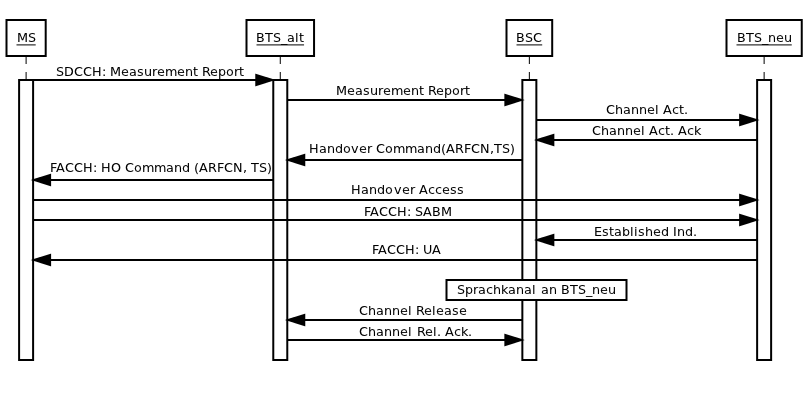
\includegraphics[width=\textwidth]{img/ablauf_handover}
  \caption{Ablaufdiagramm eines Intra BSC Handover}
  \label{fig:adhandover}
\end{figure}

Abbildung \ref{fig:adhandover} zeigt das Ablaufdiagramm eines Intra BSC Handover. Nach der Entscheidung des BSC einen Handover durchzuführen, wird im ersten Schritt ein TCH in der neuen BTS aufgebaut. War dieser Vorgang erfolgreich, wird der Mobile Station über den FACCH der bestehenden Verbindung ein Handover Command übermittelt. Das Handover Command enthält als Parameter die Frequenz und den Timeslot des TCH der neuen BTS. Nach der Synchronisation der Mobile Station mit der neuen BTS, sendet es in vier aufeinanderfolgenden Bursts eine Handover Access Message und anschließend eine Set Asynchronous Balanced Mode Message. Die neue BTS quittiert den erfolgreichen Handover mit einem Established Indicator gegenüber dem BSC und einer UA Massage gegenüber der Mobile Station. Nachdem der BSC die Verbindung auf den neuen TCH umschaltet, wird der TCH in der alten BTS abgebaut. Der Handover Vorgang ist damit abgeschlossen. Die wichtigesten Punkte für die Analyse bzw. Impelmentierung einer Handover-Funktionalität sind damit:

\begin{itemize}
 \item Erfassung und Auswertung der Measurement Reports
 \item Logik für die Entscheidungsfindung eines Handover
 \item Inter BTS Kommunikation zum Aufbau eines neuen TCH
 \item Erzeugen und Senden eines Handover Command
 \item Umschalten der bestehenden Verbindung und Abbau des alten TCH
\end{itemize}

\subsection{Projektziel und -durchführung}

%TODO: Gefällt mir noch nicht so richtig

Ziel der Projektarbeit ist die Integration der in Abschnitt \ref{sec:handover} eingeführten Handover-Funktionalität in die Open Source Software OpenBTS. Das OpenBTS Projekt ermöglicht, zusammen mit einer entsprechenden Radio-Hardware und zusätzlichen Software-Komponenten (GNURadio und Asterisk), den Betrieb eines GSM-Netzwerks. Mit der kommerziell vertriebenen Version der Software ist ein Handover zwischen zwei BTS möglich. Die Vorraussetzungen für eine erfolgreiche Integration eines Handover Moduls sind somit gegeben. Die Architektur, Installation und Konfiguration des verwendeten OpenBTS-Systems werden in Kapitel \ref{sec:openbts} ausführlich beschrieben.

Noch vor der Integrations- und Implementierungsphase wird der Ablauf eines Handover genauer analysiert. Zu diesem Zweck wird ein OpenBSC-System aufgesetzt, mit dem das in Abschnitt \ref{sec:handover} eingeführte Handoverszenario reproduziert werden kann. Die Architektur und Konfiguration des OpenBSC-Systems für die Durchführung eines Intra BSC Handover werden in Kapitel \ref{sec:openbsc} behandelt.

Da es keine brauchbare Dokumentation zur Implementierung von OpenBTS gibt enthält Kapitel \ref{} einen Überblick zur Software-Architektur und detaillierte Beschreibungen zu verwendeten Klassen des OpenBTS-Quellcodes. Der Architekturentwurf für die Integration und die durchgeführten Implementierungsarbeiten des Handover-Moduls werden in Kapitel \ref{sec:erweiterung} behandelt.

Die Analyse der durchgeführten Handover (sowohl mit OpenBSC als auch mit OpenBTS) erfolgt mit Hilfe der auf der Um- und Abis-Schnittstelle erstellen Wireshark Traces und ist in Kapitel \ref{sec:analyse} beschrieben.
